\begin{figure}
    \centering
    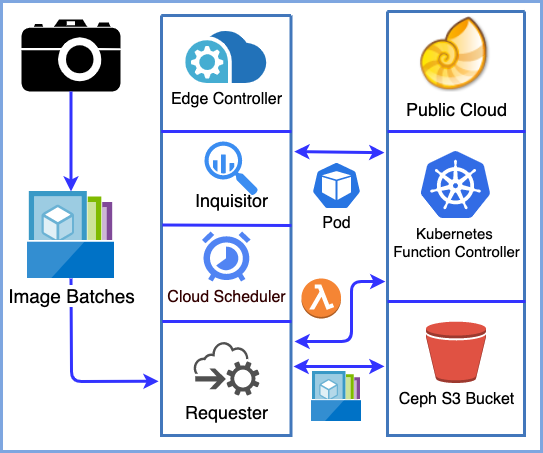
\includegraphics[scale=0.5]{figures/STOIC.png}
    \caption{The STOIC Architecture \label{fig:STOIC}}
\end{figure}


To leverage hardware acceleration and distributed scheduling within a serverless architecture, we have developed STOIC, a framework for distributing and executing analytics applications across multi-tier IoT (sensing-edge-cloud) settings. Specifically, STO\-IC optimizes the end-to-end process of packaging, transferring, scheduling, executing, and result retrieval for machine learning applications in these settings.  

Figure~\ref{fig:STOIC} shows the distributed components of STOIC. At the edge, STOIC gathers application input data, determines whether the lower application latency will be achieved by processing the data on the edge or in the cloud, and then actuates the application's computation (with the necessary data) using the ``best'' choice. The public cloud component manages whatever cloud resources are needed to receive the data from the edge, trigger the computation, and return the results to the edge.  The edge and cloud systems mirror each other, running Kubernetes~\cite{ref:k8s-web,ref:k8s} overlaid with kubeless~\cite{ref:kubeless}, to provide a uniform infrastructure for the framework.

Our system design is motivated by a need to classify wildlife images in a location where it is possible to site a relatively powerful edge system but where network connectivity is poor.  In this paper, we report on the use of STOIC  for processing images from multiple, motion-triggered camera traps (sensors) deployed to a wildlife preserve currently used to study ecological land use.
%monitor wildlife across the Sedgwick Natural Reserve~\cite{ref:sedgwick}.

\subsection{Edge Controller} 

The STOIC edge controller is a server that runs in an
outbuilding at the reserve. It communicates wirelessly with the sensors and triggers analysis and computation upon their arrival. The edge controller is connected to a research facility (which has full Internet connectivity) 
%remove for blind: the UCSB campus
via a microwave link. When a camera trap detects motion, it takes photos and persists the images in flash storage buffer, where human experts would label images for training tasks. Periodically, sensors transfer saved photos to the edge controller. During a transfer cycle, the edge controller compresses and packages all images generated and transfers the package to the public cloud, if/when necessary. STOIC runs on the edge controller and its execution is triggered by the arrival of image batches. 

As an intermediate computational tier between the sensors and the public cloud, the edge controller can be placed anywhere, preferably near the edge devices, to lower the response latency for the data processing and analytics applications. It consists of three major components: 
\begin{itemize}
\item The \textbf{cloud scheduler} predicts the total latency based on historical measurements for each available runtime. 
\item The \textbf{requester} takes as input the runtime and cloud predicted by the scheduler to have the least latency.  The requester stores the image package in an object storage service running in this cloud. It then triggers a serverless function (running in a Kubernetes pod) via a RESTful HTTP request to process the images.
%public cloud. If the public cloud is chosen, the requester
%first transfers the image batch to a dedicated Ceph~\cite{ref:ceph} 
%S3 bucket in the public cloud. 
\item The \textbf{inquisitor} monitors public cloud deployment time. To enable this, it periodically in the background deploys each runtime (using Kubernetes pods~\cite{ref:pods}) and records the deployment times in a database. No task/process is executed in this process (the runtime is simply deployed and taken down). We use the inquisitor to establish the historical time series for predicting the deployment latency of remote runtimes.
\end{itemize}

The edge cloud that we use in this study is deployed at a research reserve and is connected via the Internet.  It consists of a cluster of three Intel NUCs~\cite{ref:nucs} (6i7KYK), each with two Intel Core i7-6770HQ 4-core processors (6M Cache, 2.60 GHz) and 32GB of DDR4-2133+ RAM connected via two channels. The cluster is managed using the Eucalyptus cloud system~\cite{ref:euca}, which mirrors the Amazon Web Services (AWS) interfaces for Elastic Compute Cloud (EC2) to host Linux virtual machine (VM) instances and Simple Storage Service (S3) to provide object storage. The STOIC edge runtime uses Kubernetes and kubeless for serverless function execution and S3 (i.e. walrus) for object storage on the edge cloud.
 
\subsection{Public/Private Cloud}

To investigate the use of the serverless architecture with hardware acceleration, we employ a shared, multi\-university, GPU cloud, called Nautilus~\cite{ref:nautilus}, as our remote cloud system. Nautilus is an Internet-connected, HyperCluster research platform developed by researchers at UC San Diego, the National Science Foundation, the Department of Energy, and multiple, participating universities globally.  Nautilus is designed for running data and computationally intensive applications. It uses Kubernetes~\cite{ref:k8s} to manage and scale containerized applications. It also uses Rook~\cite{ref:rook} to integrate Ceph~\cite{ref:ceph} for object storage. As of May 2020, Nautilus consists of 176 computing nodes across the US and a total of 543 GPUs in the cluster. All nodes are connected via a multi-campus network. In this study, we consider Nautilus a public cloud that enables us to leverage hardware acceleration (GPUs) in the serverless architecture. The STOIC cloud/GPU runtimes use Kubernetes and kubeless for serverless function execution and Ceph for object storage on the public cloud.

A major challenge that we face with such deployments is hardware heterogeneity and performance variability. On Nautilus, we have observed 44 different types of CPU (e.g. Intel Xeon, AMD EPYC, among others) and 9 GPU types (e.g. Nvidia 1080Ti, K40, etc.). Both CPUs and GPUs of different types have different performance characteristics. Moreover, the object storage service is run on dedicated nodes that are distributed globally.

This heterogeneity impacts application execution time (which STOIC attempts to predict) in three significant ways. First, different CPU clock rates affect the transfer of datasets from the main memory to GPU memory. Second, there is significant latency and performance variability between runtimes and the storage service (which hold the datasets and models). Third, the multi-tenancy of nodes (common in public cloud settings) allows other jobs to share computational resources with our applications of interest at runtime. 

These three factors negatively make it difficult for users to determine which runtime to use (to reduce application turn-around time) and when to execute locally (avoiding public  cloud use altogether). With STOIC, we address these challenges via a novel scheduling system that adapts to this variability. In our results, we ensure reproducibility (avoiding network performance variability) by confining nodes and GPUs (still heterogeneous) to a single Nautilus region.

\subsection{Runtime Scenarios}

To schedule machine learning tasks across hybrid cloud deployments, we define four runtime scenarios: \textbf{(A)} \textit{Edge} - A VM instance on the edge cloud with AVX2~\cite{ref:avx} support; \textbf{(B)} \textit{CPU} - A Kubernetes pod on Nautilus containing a single CPU with AVX2 support~\cite{ref:avx}; \textbf{(C)} \textit{GPU1} - A Kubernetes pod on Nautilus containing a single GPU; \textbf{(D)} \textit{GPU2} - A Kubernetes pod on Nautilus containing two GPUs.  STOIC considers each of these deployment options as part of its scheduling decisions. Users can parameterize STOIC with their choice of deployment or allow STOIC to automatically schedule their applications.

\subsection{Execution Time Estimation}

As depicted in Figure~\ref{fig:STOIC}, the STOIC's edge controller listens for image batches from the remote camera traps and makes machine learning job requests. After a preset period (parameterizable but currently set to an hour), STOIC estimates total response time~($T_s$) of a requested batch, based on 4 different runtime scenarios. The total response time ($T_s$) includes data transfer time~($T_t$), runtime deployment time~($T_d$), and the corresponding processing time~($T_p$). We define total response time~($T_s$) as $T_s = T_t + T_d + T_p$.
 
\subsubsection{Transfer time ($T_t$)} 

$T_t$ measures the time spent in transmitting a compressed batch of images from the edge controller to edge cloud and public cloud. We calculate transfer time as ${T_t = F_b / B_c}$ where $F_b$ represents the file size of batch and $B_c$ represents the bandwidth at the moment provided by a bandwidth monitor at the edge controller. 
 
\subsubsection{Runtime deployment time ($T_d$)} 

$T_d$ measures the time Nautilus uses to deploy requested kubeless function. Since the scarcity of computation, it is common that multi-GPU runtime takes longer to deploy than single-GPU and CPU runtimes. Note that, for \textit{edge} runtime, the deployment time zeroes out since STOIC executes the task locally in the edge cloud.
 
\begin{figure*}
    \centering
    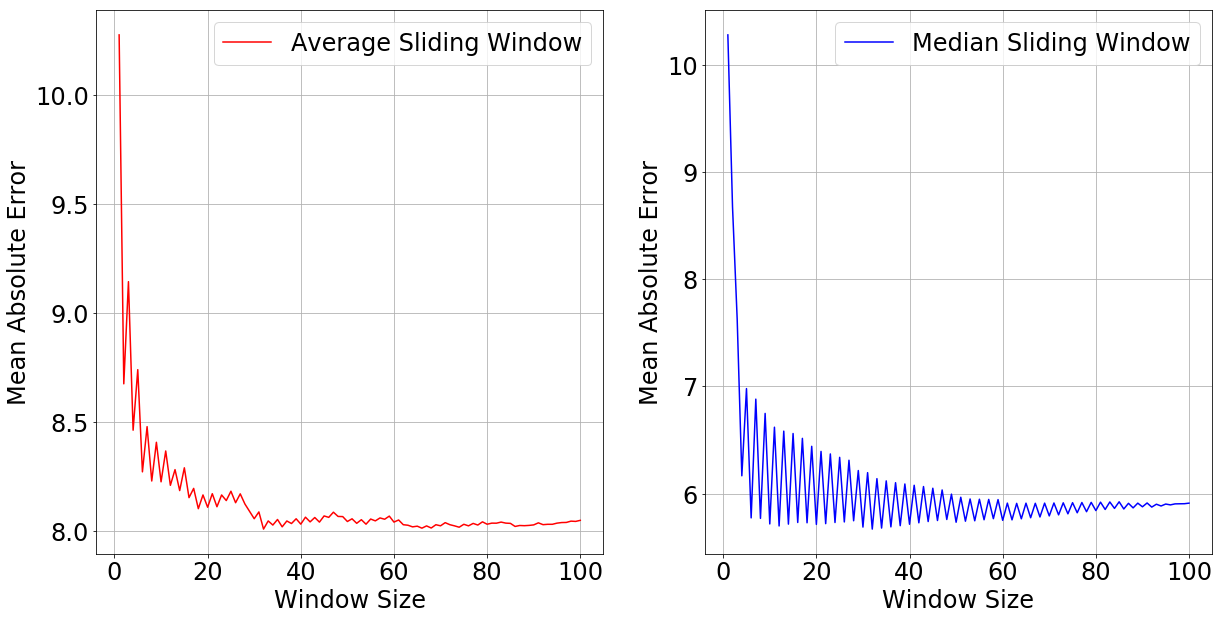
\includegraphics[scale=0.31]{figures/deployment}
    \caption{The Mean Absolute Error (MAE) of deployment time for the GPU1 runtime. The x-axis is the window (history) size. The left subplot is MAE when STOIC uses the average sliding window, the right subplot is MAE when STOIC uses the median sliding window.
\label{fig:deployment}}
\end{figure*}

 
\begin{table}
\centering
\resizebox{320pt}{!}{
\scriptsize
\resizebox{\columnwidth}{!}{
\begin{tabular}{|c|c|c|c|} 
\hline
& & \textbf{Optimal} & \textbf{Minimum}  \\
\textbf{Modeling} & \textbf{Runtime} & \textbf{Window Size} & \textbf{MAE}  \\
\hline
AutoReg & CPU & 15 & 8.977 \\
\hline
AutoReg & GPU1 & 15 & 9.605 \\
\hline
AutoReg & GPU2 & 15 & 17.918 \\
\Xhline{2\arrayrulewidth}
Avg. SW & CPU & 33 & 7.714 \\
\hline
Avg. SW & GPU1 & 31 & 8.006 \\
\hline
Avg. SW & GPU2 & 91 & 16.52 \\
\Xhline{2\arrayrulewidth}
Med. SW & CPU & 13 & \textbf{5.96} \\
\hline
Med. SW & GPU1 & 31 & \textbf{5.668} \\
\hline
Med. SW & GPU2 & 27 & \textbf{14.48} \\
\hline
\end{tabular}
}
}
\caption{Mean Absolute Error of three time series modeling methods for runtime deployment time: auto-regression (AutoReg), average sliding window (Avg. SW), and median sliding window (Med. SW). The median sliding window achieves the lowest minimum MAE at optimal window size (that with the lease MAE) for all three runtimes. \label{tab:deployment}}

\end{table}
 

Because Nautilus is a shared cloud system, we observe significant variation in deployment time on Nautilus for different times of the day. To accurately predict deployment time, we analyze deployment times as a time series using three methods: (1) auto-regression modeling, (2) average sliding window, and (3) median sliding window. Auto-regression~\cite{ref:autoreg} is a time series modeling technique based on the auto-correlation between previous time steps and the following ones. The average sliding window is the moving average~\cite{ref:moveavg} scanning through the time series by a fixed-length window. Similarly, the median sliding window captures the moving median cross the time series. All window sizes used for three modeling processes are optimized based on historical data of deployment time~($T_d$) in January 2020. We then compare the minimum Mean Absolute Error (MAE) from each to select the best modeling methodology. 

In this example, we consider a time series of 1244 data points for each runtime. Figure~\ref{fig:deployment} shows representative analytics for GPU1 deployment time, in which MAE oscillates as window size varies. We observe that the median sliding window reaches a lower minimum MAE than the average sliding window at optimal window size. As listed in Table~\ref{tab:deployment}, all three runtimes achieve the lowest minimum MAE using the median sliding window. Therefore, STOIC adopts this methodology for deployment time prediction. 

The inquisitor measures and records deployment time for each public cloud runtime every minute (called the inquisitor period). After the inquisitor records 10 new measurements (called the calibration period), the scheduler recomputes the window size over the previous 100 measurements that result in the minimum MAE. It then uses this minimum MAE window size to estimate of deployment time when jobs arrive. The inquisitor period, calibration period, and maximum window size are all modifiable.
%explain here how STOIC uses this data to adapt window size and when the estimate
%is computed.  Is this estimate what is used by the scheduler?
%%STOIC slides this window as new deployment measurements are logged by the
%%inquisitor.  The default window size in our experiments is 100 
%%measurements; STOIC calculates a
%%new estimate every 10 measurements. Both of these parameters are modifiable.

%The number of data points
%used in the analysis (i.e. 100 by default) and the interval of calibration (i.e.
%every 10 executions by default) are both parameterizable, to allow for
%tuning and trading off performance and accuracy. By default (used in our 
%results), the inquistor
%measures deployment time of the public cloud runtimes every minute.
%CJK
 
\subsubsection{Processing time~($T_p$)} 

$T_p$ is the execution time of a specific machine learning task and the target of task scheduling across the hybrid cloud. STOIC formulates a linear regression on execution time histories of STOIC jobs, and uses it to predict processing time relative to input (image batch) size. Specifically, we use Bayesian Ridge Regression~\cite{ref:brr} due to its robustness to ill-posed problems (relative to ordinary least squares regression~\cite{ref:ols}). STOIC queries the database for the most recent processing time data (e.g. 10 data points) for each regression. This ensures that the parameters of the regression line reflect the current runtime performance.

\begin{algorithm}[]
\caption{Random Sample Consensus}
\label{algo:ransac}
\SetAlgoLined
\KwData{
(1) Observation set of Process time $T_p$\\
(2) Bayesian Ridge Regression model $M$\\
(3) Minimum sample size $n$\\
(4) Residual threshold $t$\\
(5) Maximum iteration $k$ \\
(6) Required inlier size $d$ \\ 
(7) Minimum Root Mean Square Error $e$ \\
}
\KwResult{A set of parameters that best fits the data}
 \While{iterations $\leq$ k}{
    curr\_sample := $n$ data points from observation\;
    curr\_model := $M$ regressed on curr\_sample\;
    fit\_data := empty set\;
    \For{ every data point $p$ in curr\_sample}{
        \uIf{error of $p$ $\leq$ $t$}{
            $p$ $\to$ fit\_data\;
        }
    }
    \eIf{fit\_data size $\geq$ $d$}{
        curr\_error := average error in fit\_data\;
        \uIf{curr\_error < $e$}{
            Update $M$ and $e$
        }
    }{Increment iteration}
 }
 return $M$
\end{algorithm}
 
As part of our investigations into this approach, we have found that this approach is highly susceptible to outliers. The root cause of these outliers is sporadic congestion and maintenance (for nodes, networking, etc.) of the public cloud. Deviating significantly from the average, outliers skew the regression line and overestimate the runtime latency for extended periods (due to the windowing approach). We thus augment regression using a random sample consensus (RANSAC) technique~\cite{ref:ransac}, which iteratively removes outliers from the regression. The algorithm~\ref{algo:ransac} illustrates our RANSAC approach in STOIC.

 
 \begin{figure*}
    \centering
    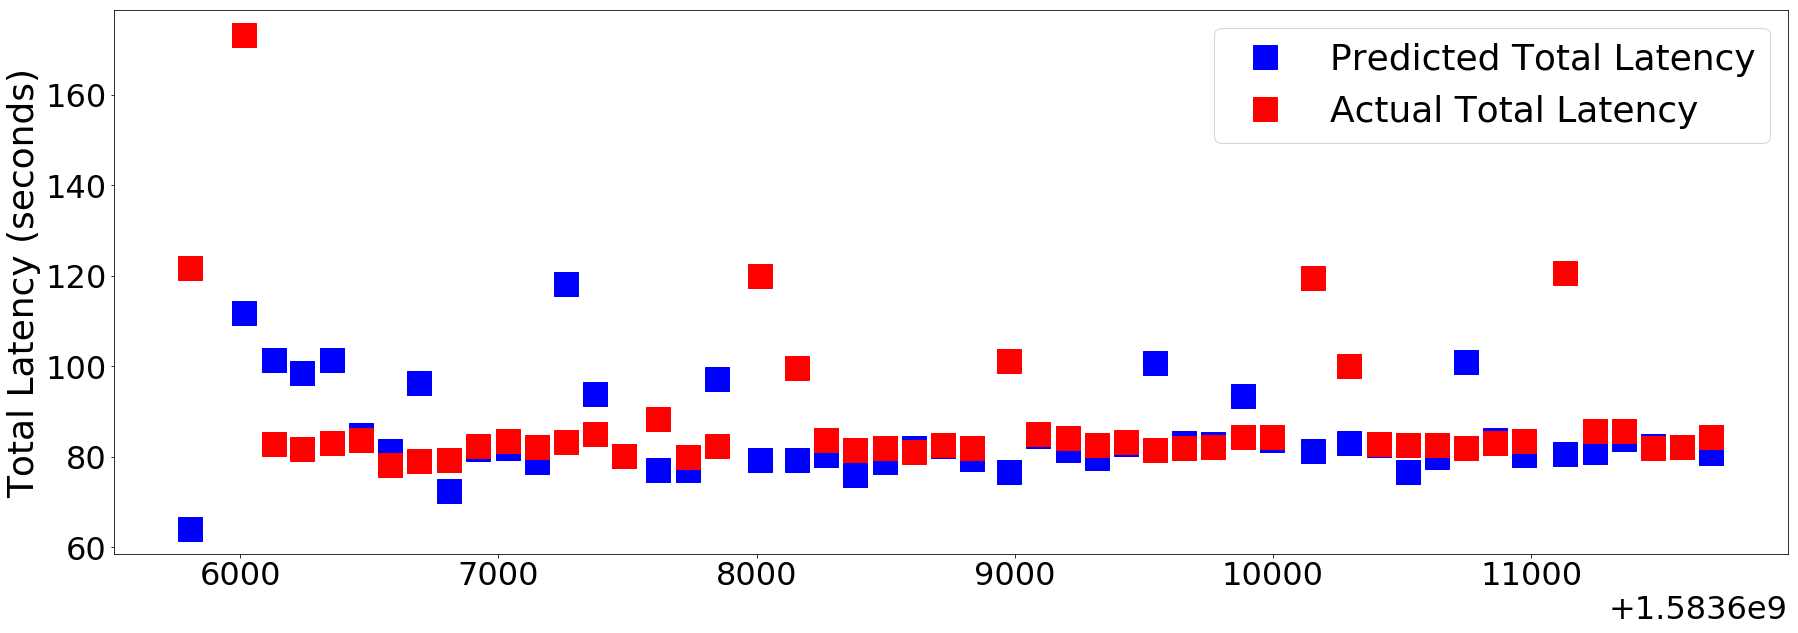
\includegraphics[scale=0.20]{figures/timeline.png}
    \caption{The comparison of predicted and actual total latency on 50 GPU1 benchmark executions with 150-image batch size. The x-axis is the epoch time and the y-axis is the total latency. \label{fig:timeline}}
\end{figure*}

\begin{table}
\centering
\resizebox{340pt}{!}{
\scriptsize
\resizebox{\columnwidth}{!}{
\begin{tabular}{|c|c|c|c|} 
\hline
 & \textbf{Deployment $T_d$} & \textbf{Processing $T_p$} & \textbf{Total $T_s$}  \\
\hline
First Half & 42.7\% & 11.2\% & 15.8\% \\
\hline
Second Half & 29.2\% & 5.3\% & 9.2\% \\
\hline
\end{tabular}
}

}
\caption{The percentage mean absolute error (PMAE) of deployment, processing, and total latency. PMAE is a latency-normalized metric and calculated as MAE divided by mean latency, which indicates the residual in a measured period. The decline of three latency metrics in the second half demonstrates the adaptability of STOIC.
\label{tab:timeline}}
\end{table}
 
 \subsubsection{Adaptability}
 
To verify that STOIC's estimation of execution time captures the actual latency of the public cloud, we execute the application 50 times with 150-image batch using the GPU1 runtime. Depicted in Figure~\ref{fig:timeline}, we observe that actual total latency varies significantly and predicted total latency has a non-negligible difference from the actual total latency at the beginning of the experiment. However, over time, as STOIC learns the various latencies of the system, the difference is significantly reduced. In Table~\ref{tab:timeline}, we report the percentage mean absolute error (PMAE), which we compute as the MAE divided by mean latency. The decrease in all three PMAE values in the second half of the execution trace also show STOIC's adaptability.

\begin{figure*}
\centering
\begin{minipage}{.45\textwidth}
  \centering
  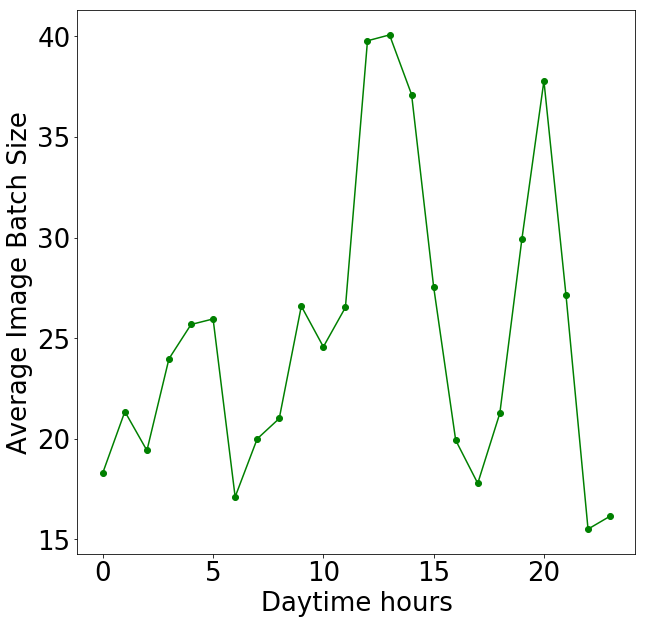
\includegraphics[width=\linewidth]{figures/Hourly_act.png}
\end{minipage}%
\hspace{0.5in}
\begin{minipage}{.45\textwidth}
  \centering
  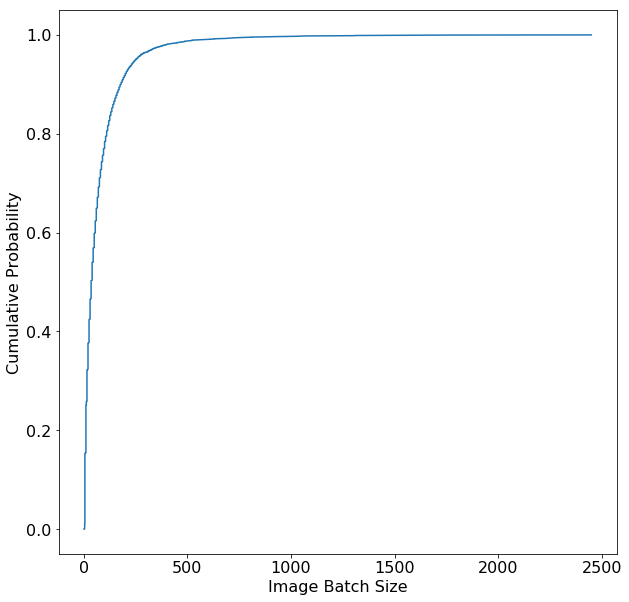
\includegraphics[width=\linewidth]{figures/ecdf.png}
\end{minipage}
\caption{Wildlife Hourly Activity Level (left graph) and its Conditional Empirical Cumulative Distribution Function (right graph). The left graph demonstrates the mean activity level of wildlife throughout the daytime. Based on the curve, 1 PM and 8 PM are two peak hours of animal activities.  The right graph shows the empirical CDF, which STOIC randomly samples for image batches to drive our faster-than-real time empirical evaluation of the system.\label{fig:hour_act_and_cdf}}
\end{figure*}

\ignore{
\begin{figure*}[t] \centering 
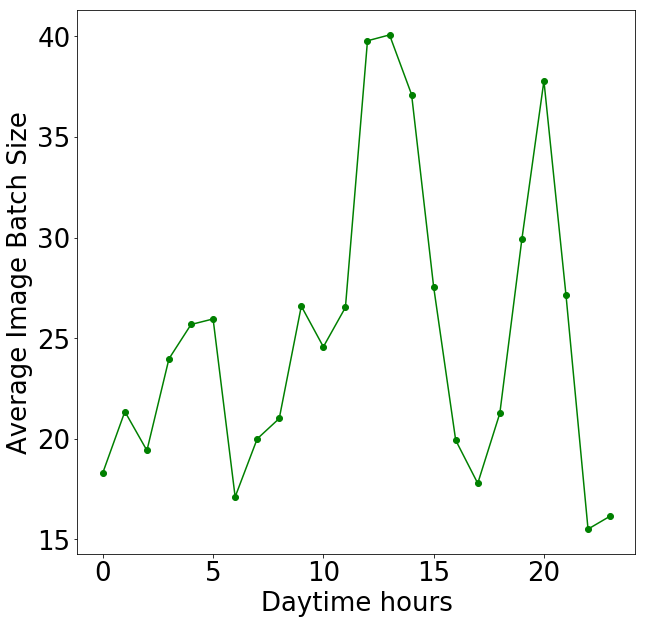
\includegraphics[scale=0.4]{figures/Hourly_act.png}
\caption{Wildlife Hourly Activity Level. The figure demonstrates the mean activity level of wildlife throughout a day. Based on the curve, 1PM and 8PM are two peak hours of animal activities.
\label{fig:hour_act}}
\end{figure*} 
 
 
\begin{figure*}[t] \centering 
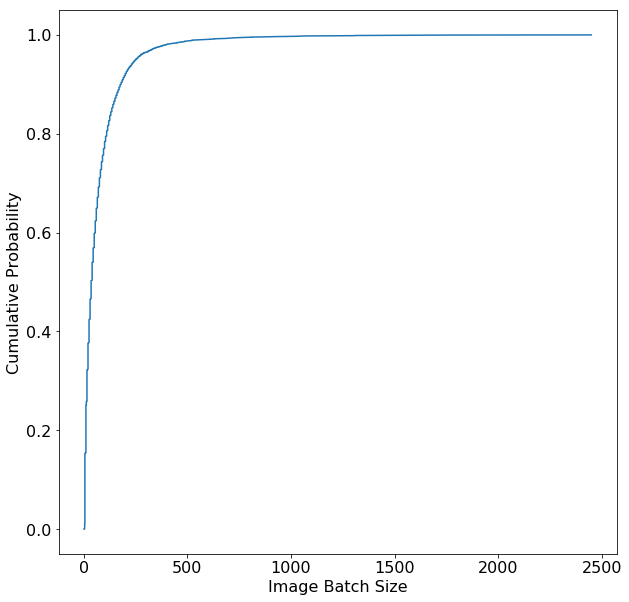
\includegraphics[scale=0.4]{figures/ecdf.png}
\caption{Conditional Empirical Cumulative Distribution Function. The STOIC image batch simulator is based on this function and random probabilities [0, 1) from a uniform distribution.
\label{fig:cecdf}}
\end{figure*} 
}
 
\subsection{Workload Generation}
\label{sec:workloadgen}

To drive our empirical evaluation in faster-than-real time,  we construct a workload generator from image batch histories (traces) collected by our camera traps. We consider the set of images that occur together within an hour (i.e. due to motion events) a batch. Our camera trap trace, starting on July 13th, 2013 and ending Jan. 15th, 2017, comes from a fixed camera located at a watering hole in a remote area of our research reserve. The trace contains images of bear, deer, coyote, puma, and birds as well as wind-triggered empty images and other animals.

After excluding camera maintenance periods (gaps), we  extract 1136 effective days (27264 hours) of data. The maximum size of hourly image batch is 2450, whereas the minimum size is unsurprisingly zero, which constitutes 18139 hours out of 27264 hours (66.53\%). On average, an hourly image batch size contains 25 images. The left graph in Figure~\ref{fig:hour_act_and_cdf} illustrates the wildlife  hourly activity level based on the image batch size. We infer from the curve that 1 PM and 8 PM are two peak hours of animal activity.

Specifically, we construct a conditional empirical cumulative distribution function~(ECDF) based on the probability definition of  $Pr(x < K | x > 0)$, where x is the image batch size and K is the cutoff value. This conditional ECDF effectively represents the trajectory of the animal activity level and makes the evaluation empirical. The right graph in Figure~\ref{fig:hour_act_and_cdf} plots the conditional ECDF. 
The x-axis is the image batch size ranging from zero to 2450, whereas the y-axis is the cumulative probability. The STOIC workload generator draws image batch sizes by
randomly sampling this ECDF.
%The sampling procedure is as follows.  During the execution of STOIC, 
%the simulator first generates a
%random number in [0, 1) from a uniform distribution and secondly retrieves the
%corresponding image batch size from the conditional ECDF. 
Using this process, we are able to evaluate and conclude by replaying the image stream from the camera traps in fast-than-real time for the purposes of comparative evaluation.

%, regarding STOIC's
%performance and efficiency by a real-world streaming data flow.



 \subsection{Implementation}

%Considering performance and interface, 
We implement STOIC using Golang~\cite{ref:golang}. Golang provides high-performance execution (vs scripting languages) and a user-friendly interface~\cite{ref:client-go} to Kubernetes and database technologies. STOIC currently supports machine learning applications developed using the TensorFlow framework~\cite{ref:tensorflow} and can be easily extended to permit other machine learning libraries.
%by extending the runtime
%environment.
 
As mentioned previously, the STOIC serverless architecture leverages kubeless~\cite{ref:kubeless}. As a Kubernetes-native serverless framework, kubeless uses the Custom Resource Definition (CRD)~\cite{ref:crd} to dynamically create functions as Kubernetes custom resources and launches runtimes on-demand. For specific machine learning tasks that STOIC executes, we build custom Docker images that we upload to Docker Hub~\cite{ref:dockerhub} in advance. When the function controller receives a task request, it pulls the latest image from Docker Hub before launching the function. This deployment pipeline makes the runtime flexible and extensible for evolving applications. 
%To create a consistent serverless environment, we install and configure
%minikube~\cite{ref:minikube} and kubeless~\cite{ref:kubeless} on the edge
%cloud. They enable the edge cloud to execute and respond to serverless
%function requests in the same manner as Nautilus. To further reduce the
%deployment time on the minikube cluster, 

To leverage the computational power of our CPU systems, we compile Tensorflow with AVX2, SSE4.2 \cite{ref:avx} and FMA~\cite{ref:fma} instruction set support. We use this optimized version of Tensorflow on both the edge and public clouds.
%From our previous test result
%in~\cite{ref:stoic}, we observe significant speed-up from the customized
%library on CPU runtime. Therefore, we use this Tensorflow configuration on
%both the edge cloud and Nautilus.
 
To enable GPU access by serverless functions (available in the public cloud), we equip our Docker container with NVIDIA Container Toolkit~\cite{ref:nvidia}. This includes the NVIDIA runtime library and utilities, which link serverless functions to NVIDIA GPUs. We also install CUDA 10.0 and cuDNN 7.0 to support the machine learning libraries.
 
 
 \subsection{Workflow}

\begin{figure}[t] \centering 
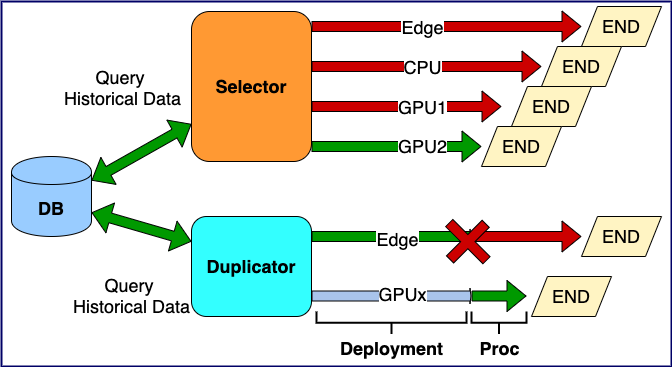
\includegraphics[scale=0.5]{figures/selector_duplicator.png}
\caption{The selector and duplicator modes of STOIC. 
\label{fig:duplicator}}
\end{figure}


STOIC considers two workflows upon receiving an image batch: 
selector mode and duplicator mode. Both are depicted in Figure~\ref{fig:duplicator}. In selector mode, STOIC predicts the total response times~($T_s$) of the four deployment options: Edge, CPU, GPU1, and GPU2.  It then selects the runtime with the shortest estimated response time and deploys it locally (Edge) or remotely (non-Edge). Once deployed, the pod notifies the STOIC requester at the edge which then triggers the serverless function via an HTTP request. When the task completes, the pod notifies the requester, which retrieves the results and runtime metrics from the deployment and stores them in the database for use by the scheduler.

To handle deployment failure, STOIC implements a retry mechanism using exponential back-off. Starting at 100 milliseconds, STOIC waits 2X length of time for retrying the deployment on Nautilus. After 10 failed attempts, STOIC claims timeout and returns an error.

STOIC also attempts to reduce startup time (i.e. cold starts) at both the edge and public cloud. On the edge cloud, STOIC creates a standby pod to serve the incoming request upon application invocation. On the public cloud, STOIC triggers a function with a single image to retrieve and cache the base model in memory at each pod.
 
%Once Nautilus successfully deploys the serverless function, it informs the
%edge cloud's requester to trigger the function via an HTTP request. To cope
%with the cold starts~\cite{ref:coldstart}, STOIC triggers the function with
%the least amount of input data to ensure the function caches the model in
%memory. When the task completes, the requester retrieves the results and
%runtime metrics, and transmits them back to the edge controller. Finally, the
%edge cloud logs the results and metrics to the database for use in later
%predictions. 

We observe from Table~\ref{tab:timeline} that there are significant variations in the deployment time of the runtimes on the shared public cloud. To enable STOIC to adapt to this variability, we consider a second workflow called \textbf{duplicator} mode. Using this mode, when the scheduler selects a public cloud runtime (i.e. CPU, GPU1, GPU2), the requester \textit{also} deploys the job on the edge cloud. It then terminates edge cloud execution if the remaining time at edge cloud is longer than the expected processing time ($T_p$) at the GPU runtime once deployment completes. This ``lagging decision'' mechanism reduces the variability of deployment time in the prediction. As a result, STOIC must only consider processing time, which is more accurately predicted, to deploy tasks. Note that duplicator mode is less energy-efficient because it runs tasks regardless of latency prediction and may waste cloud resources by killing the function in the middle. However, if such waste can be tolerated, significant prediction accuracy and latency reduction are possible.

In addition, the inquisitor running in background deploys the public cloud runtimes periodically and stores the deployment time duration in the database for use in the prediction. We set a timeout (i.e. 10 minutes) to terminate this process for any unresponsive deployment. That is, the inquisitor marks the runtime unavailable (from the point of view of the requester) when the deployment hits the set timeout. The inquisitor continues to attempt deployment of this runtime periodically and makes it available to the requester once a deployment attempt is successful.

To bootstrap the system, STOIC executes two representative tasks for an application for each runtime in both the edge and public cloud. It uses these data points as a basis for its processing time estimation by linear regression. STOIC performs this bootstrapping each time a new version of the application is uploaded by the developer.

%Extended from the initial version, we enable STOIC to take application name
%and versioning information as input. Once a new application is deployed or the
%existing application is updated, the regression initiator automatically
%executes two tasks based on the current application and version for each
%runtime scenario. These two data points 
%initialize the incoming regressions
%and predictions across the edge and public cloud.

%. Seen in Figure~\ref{fig:duplicator}, the
%edge cloud then schedules only one request, using the payload of
%compressed image batch and runtime information. Upon execution, the edge cloud
%triggers the serverless function locally if/when the choice is the \textit{edge}
%runtime. %Edge deployment is typically selected when batch size is small. 

%For large batch sizes, STOIC typically schedules one of the three public
%runtime options. For these three scenarios, the edge cloud first requests the
%deployment on the public cloud. It then sends the payload to public cloud
%storage. The public cloud then deploys the runtime on nodes that satisfy the
%node affinity configuration. 

